\section{}
\[
H(s)=\frac{-1000\,(s+2)^2}{4\,(s+1)^3\,(s+10)}=-250\,\frac{(s+2)^2}{(s+1)^3\,(s+10)}\,.
\]
\subsection{Bode-Diagramm}
\begin{center}
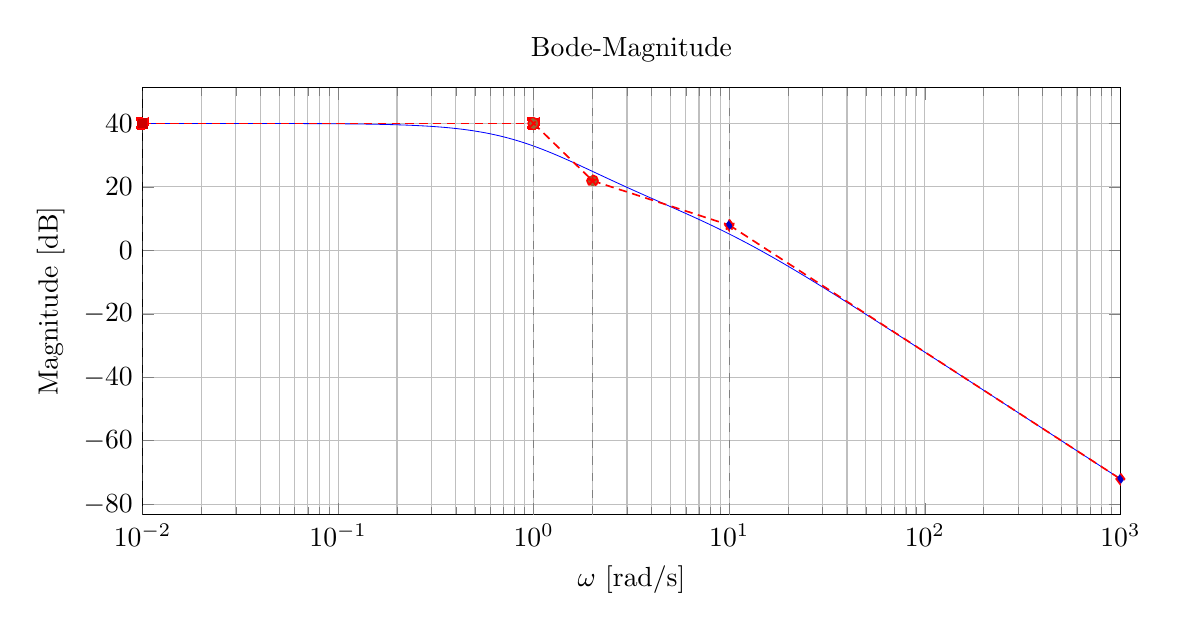
\begin{tikzpicture}
\begin{semilogxaxis}[
  width=14cm,height=7cm,
  ytick distance=20,
  xmin=1e-2,xmax=1e3,
  xlabel={$\omega$ [rad/s]},
  ylabel={Magnitude [dB]},
  grid=both,
  title={Bode-Magnitude}
]
\addplot[
  domain=1e-2:1e3,
  samples=900,
  mark=none,
  line width=0.3pt,
  blue
] {20*ln(250)/ln(10)
    +40*ln(sqrt(4 + x^2))/ln(10)
    -60*ln(sqrt(1 + x^2))/ln(10)
    -20*ln(sqrt(100 + x^2))/ln(10)};
\addplot+[domain=1e-2:1,samples=2,dashed,dash pattern=on 3pt off 2pt,line width=0.6pt,red] {40};
\addplot+[domain=1:2,samples=2,dashed,dash pattern=on 3pt off 2pt,line width=0.6pt,red] {40 - 60*ln(x)/ln(10)};
\addplot+[domain=2:1e1,samples=2,dashed,dash pattern=on 3pt off 2pt,line width=0.6pt,red] {40 - 60*ln(2)/ln(10) - 20*ln(x/2)/ln(10)};
\addplot+[domain=1e1:1e3,samples=2,dashed,dash pattern=on 3pt off 2pt,line width=0.6pt,red] {40 - 60*ln(2)/ln(10) - 20*ln(10/2)/ln(10) - 40*ln(x/10)/ln(10)};
\draw[gray,dashed] (rel axis cs:0,0) -- (rel axis cs:0,1);
\draw[gray,dashed] (axis cs:1,\pgfkeysvalueof{/pgfplots/ymin}) -- (axis cs:1,\pgfkeysvalueof{/pgfplots/ymax});
\draw[gray,dashed] (axis cs:2,\pgfkeysvalueof{/pgfplots/ymin}) -- (axis cs:2,\pgfkeysvalueof{/pgfplots/ymax});
\draw[gray,dashed] (axis cs:10,\pgfkeysvalueof{/pgfplots/ymin}) -- (axis cs:10,\pgfkeysvalueof{/pgfplots/ymax});
\node[gray,anchor=south east] at (axis cs:2,\pgfkeysvalueof{/pgfplots/ymax}) {\scriptsize Nullstelle $\omega_z=2$ (doppelt)};
\node[gray,anchor=south east] at (axis cs:1,\pgfkeysvalueof{/pgfplots/ymax}) {\scriptsize Pol $\omega_p=1$ (dreifach)};
\node[gray,anchor=south east] at (axis cs:10,\pgfkeysvalueof{/pgfplots/ymax}) {\scriptsize Pol $\omega_p=10$};
\end{semilogxaxis}
\end{tikzpicture}
\vspace{6mm}
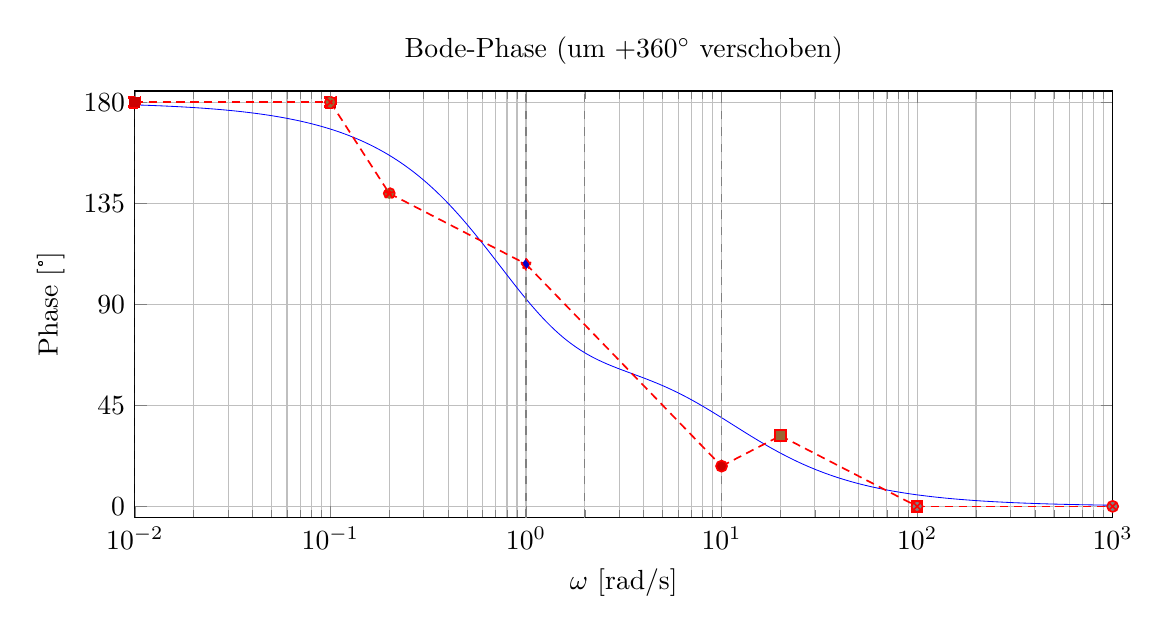
\begin{tikzpicture}
\begin{semilogxaxis}[
  width=14cm,height=7cm,
  xmin=1e-2,xmax=1e3,
  ymin=-5,ymax=185,
  ytick distance=45,
  xlabel={$\omega$ [rad/s]},
  ylabel={Phase [°]},
  grid=both,
  title={Bode-Phase (um $+360^\circ$ verschoben)}
]
% exakte (blaue) Phase: +360° Shift
\addplot[
  domain=1e-2:1e3,
  samples=900,
  mark=none,
  line width=0.3pt,
  blue
] {180 + 2*atan(x/2) - 3*atan(x) - atan(x/10)};

% rote Geradennäherung, korrekt platziert und +360° verschoben
\addplot+[domain=1e-2:1e-1,samples=2,dashed,dash pattern=on 3pt off 2pt,line width=0.6pt,red]{180};
\addplot+[domain=1e-1:2e-1,samples=2,dashed,dash pattern=on 3pt off 2pt,line width=0.6pt,red]{180 - 135*ln(x/0.1)/ln(10)};
\addplot+[domain=2e-1:1e0,samples=2,dashed,dash pattern=on 3pt off 2pt,line width=0.6pt,red]{180 - 135*ln(2)/ln(10) - 45*ln(x/0.2)/ln(10)};
\addplot+[domain=1e0:1e1,samples=2,dashed,dash pattern=on 3pt off 2pt,line width=0.6pt,red]{180 - 135*ln(2)/ln(10) - 45*ln(5)/ln(10) - 90*ln(x)/ln(10)};
\addplot+[domain=1e1:2e1,samples=2,dashed,dash pattern=on 3pt off 2pt,line width=0.6pt,red]{180 - 135*ln(2)/ln(10) - 45*ln(5)/ln(10) - 90 + 45*ln(x/10)/ln(10)};
\addplot+[domain=2e1:1e2,samples=2,dashed,dash pattern=on 3pt off 2pt,line width=0.6pt,red]{180 - 135*ln(2)/ln(10) - 45*ln(5)/ln(10) - 90 + 45*ln(2)/ln(10) - 45*ln(x/20)/ln(10)};
\addplot+[domain=1e2:1e3,samples=2,dashed,dash pattern=on 3pt off 2pt,line width=0.6pt,red]{0};

\draw[gray,dashed] (rel axis cs:0,0) -- (rel axis cs:0,1);
\draw[gray,dashed] (axis cs:1,\pgfkeysvalueof{/pgfplots/ymin}) -- (axis cs:1,\pgfkeysvalueof{/pgfplots/ymax});
\draw[gray,dashed] (axis cs:2,\pgfkeysvalueof{/pgfplots/ymin}) -- (axis cs:2,\pgfkeysvalueof{/pgfplots/ymax});
\draw[gray,dashed] (axis cs:10,\pgfkeysvalueof{/pgfplots/ymin}) -- (axis cs:10,\pgfkeysvalueof{/pgfplots/ymax});
\node[gray,anchor=south east] at (axis cs:2,\pgfkeysvalueof{/pgfplots/ymax}) {\scriptsize Nullstelle $\omega_z=2$ (doppelt)};
\node[gray,anchor=south east] at (axis cs:1,\pgfkeysvalueof{/pgfplots/ymax}) {\scriptsize Pol $\omega_p=1$ (dreifach)};
\node[gray,anchor=south east] at (axis cs:10,\pgfkeysvalueof{/pgfplots/ymax}) {\scriptsize Pol $\omega_p=10$};
\end{semilogxaxis}
\end{tikzpicture}
\end{center}
\newpage